


% \begin{table}[tbp]
%     \centering
%     %\scriptsize
%     \begin{subtable}[t]{0.48\textwidth}
%         \centering
%         \vspace{0pt} % Ensures top alignment
%         \input{./tables/Rec_Target_downstream}  
%         \caption{\textbf{Reconstruction target downstream performance.} We compare how the reconstruction targets themselves do in the downstream task. This aims to extract how much the denoising part matters compared to the motion augmentation. PFDwT1=Positive Frame difference with current frame where T=1, PFDwT2=Positive frame difference with current frame where T=2, $\sigma$=Standard deviation over all loaded frames, $\Sigma-5\bar{I}$=Sum of 5 consecutive frames - 5 * clip mean frame, $\Sigma-3\bar{I}$=Sum of 3 consecutive frames - 3 * mean frame. PFDwT1 is highlighted in gray to indicate this is our denoising autoencoder's default target.}
%         \label{tab:target_no_denoise}
%     \end{subtable}
%     \begin{subtable}[t]{0.48\textwidth}
%         \centering
%         \input{./tables/Denoising_only_downstream}  
%         \caption{\textbf{Denoising-only downstream performance, identity target.} We compare how the Denoising Autoencoder alone, without the incorporated augmented motion, does with the combination in \cref{tab:big_table}}.
%     \end{subtable}\hfill
    
%     \vspace{1em}
%     \caption{\textbf{\NAME{} ablation experiments on CFC22.} All values are generated via the detection and tracking stages of our pipeline. All reconstruction targets are sized 1024 x 512 unless otherwise stated. We report the mAP$_{50}$ of the \emph{combined} background-subtracted and target reconstruction frames unless otherwise noted. Best values are highlighted in \textbf{bold}. Default settings are highlighted in \textcolor{lightgray}{gray}. Additional ablation experiments are in the Supplemental materials. \TODO{}}
%     \label{tab:ablations}
% \end{table}

%\begin{table*}[t]
   % \centering
   % \vspace{0pt} % Ensures top alignment
   % \resizebox{\textwidth}{!}{%
   % \input{./tables/big_results_table}  
    %}
   % \caption{\textbf{Big Results Table.} \textcolor{pink}{--training another with med-filter} \textcolor{green}{whats the difference bwteen the first 2 columns of POCUS, is BUV val or test, if there is only one thats not train change this to test}baseline refers to raw for POCUS and BUV and the CFC22++\cite{cfc2022eccv} for CFC22  }
 %   \label{tab:big_table}
%\end{table*}
\section{Results}\label{sec:results}
% this can be removed if we end up needing space
\NAME{} boost signal of objects of interest in low signal-to-noise video. It improves a range of downstream tasks in a way that is computationally less resource-intensive and yields higher performance than other denoising methods.

\begin{table}[tp]
    \centering
    \vspace{0pt} % Ensures top alignment
    \resizebox{0.4\textwidth}{!}{%
    \vspace{0pt} % Ensures top alignment
\begin{tabular}{l c c c c}
\toprule
 \textbf{Train-Time (hours)} & CFC22 & POCUS & BUV \\
\hline
N2V \cite{krull2019noise2void} &  144 & 0.75 & 1.5\\
UDVD \cite{Sheth_2021_ICCV} & 96* & 12 & 23 \\
UMVD \cite{UMVD} & 91* & 34 & 42\\
LG-BPN \cite{wang2023lgbpn} & 101 & 6 & 4 \\
\NAME{} (Ours) & \textbf{20} & \textbf{0.5} & \textbf{1}\\
% \bottomrule
\end{tabular}  
    }   
    \caption{\textbf{\NAME{} is resource-efficient during training.} Note that UDVD and UMVD (U*VD) took 8 days to train CFC22, but U*VD trained CFC22 only for one epoch. For all other datasets, U*VD both trained for 10 epochs on 2 NVIDIA RTX 4090 GPUs.}
    \label{tab:denoiser_time}
\end{table}

\subsection{Denoising Performance.} 
\NAME{} produces clear contiguous objects, where other methods do not, shown in \cref{fig:qualitative_pairs} \& \ref{fig:fish_qual_denoising}. \NAME{} is also able train to convergence in 22\% of the time of the next-quickest network-based method -- more can be seen in \cref{tab:denoiser_time}.

\begin{figure}[tp]
    \centering
    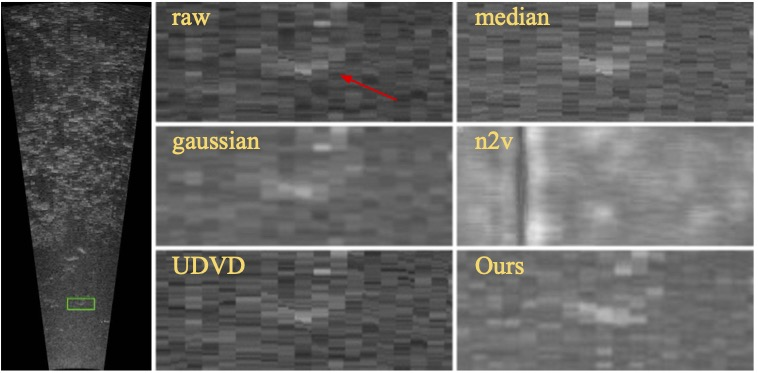
\includegraphics[width=0.75\linewidth]{figs/fish_qual_denoising.jpg}
    \caption{\textbf{Qualitative denoising performance on CFC22}. We can see that the fish is easiest to spot as a bright patch after processing with our denoiser. The green box highlights the fish location. Each denoised image zooms in to that green bounding box. The red arrow in the raw frame points to the fish location. Additional example visualizations are in \cref{fig:additional_fish_denoised} in Supp. Mat.}
    \label{fig:fish_qual_denoising}
\end{figure}

\noindent{}\textbf{Fish Denoising: CFC22.} \NAME{} increases the contrast between fish and background (\cref{fig:fish_qual_denoising}). As such, the distributions of pixel intensities at the same location when fish are present and when they are not are distinct. This is shown in \cref{tab:denoised_metrics_fish}, where \NAME{}'s $FBD$ is significantly higher than that of other methods.
\begin{table}[t]
    \centering
        \resizebox{0.35\textwidth}{!}{%
        \begin{tabular}{lcccc}
\toprule
&\multicolumn{3}{c}{$FBD$ ($\uparrow$})\\
    & Train & Val & Test  \\
    \hline
    Raw & 1005 & 652 & 860 \\
    % Background-sub & 1145 & 787.4 & 896.9\\
    CFC22++\cite{cfc2022eccv} & \textit{63.7} & 368 & 458  \\
    Median-filtered\cite{gonzalez2006meanfilter} & 523 & 334 & 364 \\
    Gaussian-filtered\cite{gonzalez2006meanfilter} & 793 & 507 & 756 \\
    N2V\cite{krull2019noise2void} & 227 & \textit{194} & \textit{180} \\
    UDVD\cite{Sheth_2021_ICCV} & 402 & 254 & 272 \\
    % Denoised {\it (framewise)} & 494 & 405 & 548\\
    \NAME{} (Ours) & \textbf{1366} & \textbf{994} & \textbf{1458}\\
    \bottomrule
\end{tabular}    
    }
    \caption{\textbf{\textit{FBD} \cref{eqn:fbd} between P(Fish) vs. Q (Non-fish).} For all ground truth bounding boxes, P and Q are composed as follows: P -- we take the set of pixels in each  box from frames with objects. Q -- we extract the set of pixels from the same box location from a frame where there is no object at that location. \textit{Raw}=raw noisy frame $I_t$, CFC22++\cite{cfc2022eccv} = 3-channel image (raw, background-subtracted, frame-to-frame difference),
    \NAME{}=denoised with motion augmentation, as in \cref{sec:reconstruction}. We calculate the KL-divergence metric, discussed in \cref{sec:KL}. $\uparrow$ indicates the metric is better the larger it is. Best values are \textbf{bolded}, worst values are in \textit{italics.}}
    \label{tab:denoised_metrics_fish}
\end{table}

\noindent{}\textbf{Fluorescent Cells Denoising: Fluo.\ } \NAME{} increases the cells' brightness relative to the background, as seen in \cref{fig:qualitative_pairs}. As is standard\cite{Sheth_2021_ICCV}, and because the data size is small, we only perform qualitative analysis on Fluo.


% \subsection{CFC22}
\subsection{Detection Performance}
\NAME{} outperforms other denoising methods when evaluated on downstream detection tasks of CFC22 and BUV.

\noindent{}\textbf{Fish Detection: CFC22.} The detection performance of \NAME{}-processed frames is better than detection performance of other processed frames for CFC22. This is shown in \cref{fig:fish_qual_denoising} \& \ref{fig:heatmaps} and  \cref{tab:big_table}. \NAME{} improves detection performance in areas where objects and signal are rare. \NAME{} frames result in an improvement of 43.2\% and 9.4\% test accuracy compared to the raw and background-subtracted frames respectively, and a 5.1\% boost in performance compared to a three-channel image (raw, background-subtracted, and frame-to-frame-absolute difference) described as baseline++ in \citet{cfc2022eccv}, but hereon referred to as CFC22++. 
\begin{table*}[htp]
    \centering
    \vspace{0pt} % Ensures top alignment
    \resizebox{0.75\textwidth}{!}{%
    \begin{tabular}{l c c c c c c c }
 \toprule
 & \multicolumn{3}{c}{CFC22 (Test)}& \multicolumn{3}{c}{POCUS (5-fold-CV)} & \multicolumn{1}{c}{BUV(Test)} \\
 \cmidrule(lr){2-4} \cmidrule(lr){5-7} \cmidrule(lr){8-8} 
 Method & mAP$_{50}$\cite{map50}$\uparrow$ & MOTA\cite{clear}$\uparrow$ & nMAE\cite{cfc2022eccv}$\downarrow$ & AP$\uparrow$ & AR$\uparrow$ & F1$\uparrow$ & mAP$_{50}$\cite{map50}$\uparrow$ \\
 \hline
\multicolumn{2}{@{}l}{\textit{Classical}} \\
Baseline  & 73.8 & 37.4 & 54.8 & 82.6 & 82.0 & 80.4 & 46.4\\
Median-Filter\cite{gonzalez2006meanfilter} & 73.7 & 37.8 & 53.0 & 86.2 & 85.5 & 85.3 & 52.4\\
Mean-Filter\cite{gonzalez2006meanfilter} & 76.4 & 44.3 & 41.4 & 84.0 & 84.7 & 83.2 & 52.6 \\
Gaussian-Filter\cite{gonzalez2006meanfilter} & 74.9 & 27.6 & 56.8 & 84.1 & 84.3 & 83.3 & 46.5 \\
\hline                    
\multicolumn{2}{@{}l}{\textit{Deep-Learning-Based Image/Video Denoising/Restoration}}                  \\  
N2V\cite{krull2019noise2void} & 67.2 & 34.2 & 34.3 & 83.7 & 82.7 & 82.4 & 46.6\\
UDVD\cite{Sheth_2021_ICCV} & 67.2 & 28.1 & 41.9 & 83.7 & 84.6 & 83.4 & 49.9 \\
UMVD\cite{UMVD} & 70.4 & 38.2 & 34.0 & 80.4 & 82.6 & 80.7 & 53.9 \\
LG-BPN\cite{wang2023lgbpn} & 72.6 & 41.9 & 34.2 & 31.9 & 34.3 & 21.5 & 49.7 \\
% \hline
% \multicolumn{2}{@{}l}{\textit{General Purpose/Blind Restoration}}   \\  
RVRT\cite{liang2022rvrt} & 62.9 & 29.3 & 43.8 & 81.8 & 79.8 & 78.7 & 26.0 \\
AverNet\cite{zhao2024avernet} & 65.4 & 30.3 & 35.7 & 83.7 & 83.4 & 82.6 & 47.0 \\

\hline                   \multicolumn{2}{@{}l}{\textit{DAEs}}          \\ 
AE & 67.8 & 34.3 & 41.7 & 82.3 & 84.7 & 82.1 & 46.9 \\
UNet \cite{unet} & 73.9 & 34.1 & 56.3 & 83.7 & 84.6 & 83.4 & 51.0 \\
UNet3D\cite{unet} & 66.9 & 32.4 & 35.4 & 83.5 & 80.1 & 80.6 & 47.6 \\
\NAME{} (Ours) & \textbf{77.6} & \textbf{47.4} & \textbf{33.9} & \textbf{87.5} & \textbf{86.7} & \textbf{86.3} & \textbf{59.5} \\
\bottomrule
\end{tabular}  
    }
    \caption{\textbf{Downstream results.} \NAME{} does well across all datasets and downstream tasks. Best performance is \textbf{bolded}. Baseline refers to raw for medical ultrasound (POCUS \cite{born2021l2, born2021accelerating} and BUV \cite{CVANet}) and the strengthened baseline CFC22++\cite{cfc2022eccv} for fish sonar (CFC22 \cite{cfc2022eccv}. AP=average precision, AR=average recall, F1=average F1, mAP$_{50}$=mean average precision of detections at IOU threshold 0.5, MOTA=Multi-Object Tracking Accuracy\cite{clear}, nMAE=normalized mean absolute counting error\cite{cfc2022eccv}. More tracking results are in \cref{fig:track}. }
    \label{tab:big_table}
\end{table*}
\begin{figure}[t]
    \centering
    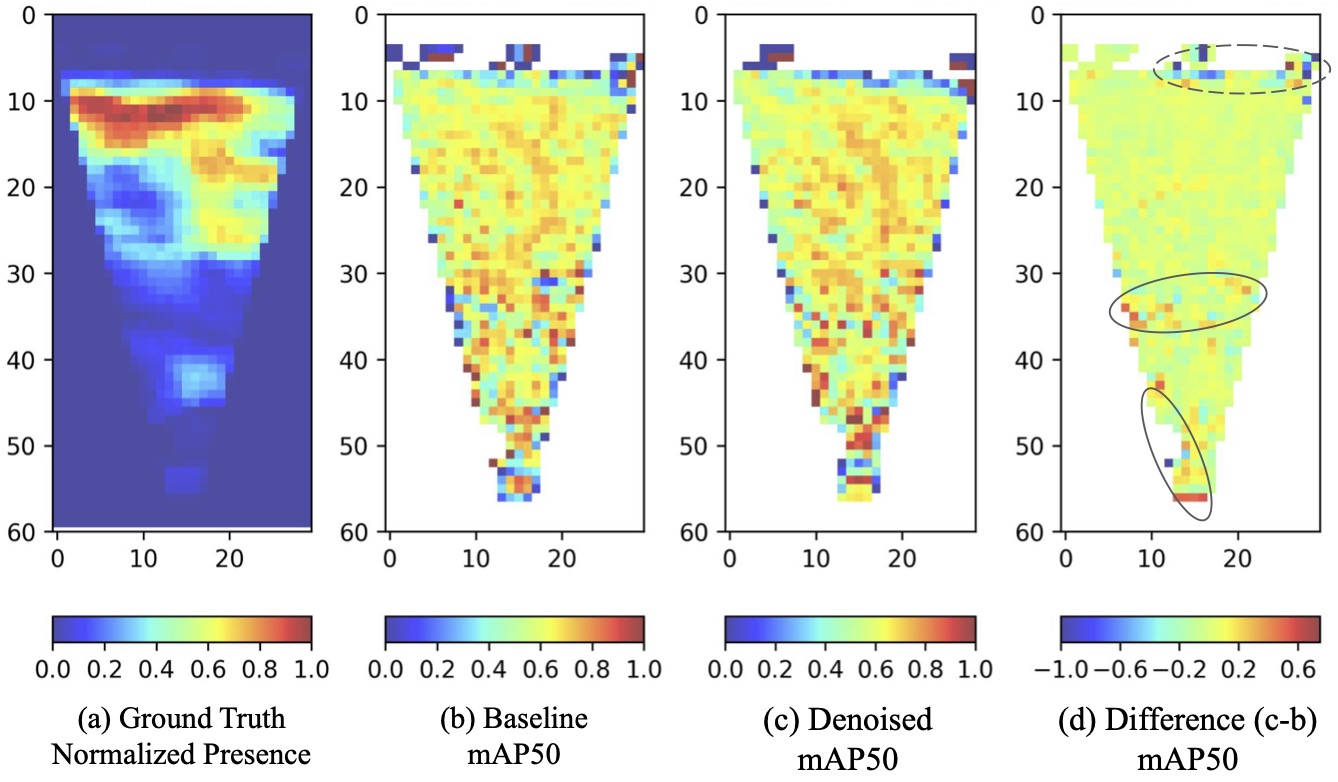
\includegraphics[width=\linewidth]{figs/patchwise_maps.jpg}
    \caption{\textbf{Denoising improves detections where signal is infrequent}. \textbf{(a)} the ground truth fish patch locations (from bounding box labels) normalized over the dataset; most fish pass by in the top region, fish crossings below are infrequent, thus there is more training signal in the top part of the videos. \textbf{(b\&c)} patchwise detection performance of CFC22++\cite{cfc2022eccv} and \NAME{}, respectively, on the CFC22 dataset. Heatmaps indicate mAP$_{50}$ performance over all frames of the test set at pixel patches. The more red a patch is, the higher the mAP$_{50}$ of that patch; the more blue the patch is, the lower the mAP$_{50}$. \textbf{(d)} the difference, \NAME{} - CFC22++, with solid ellipses at regions of heightened performance and dashed ellipses around areas of lowered performance. Denoising improves detections in areas where signal is infrequent. On the other hand, detection performance declines in areas where signal is abundant. Additional patch maps can be seen in \cref{fig:trajectory_example_with_detections} in the Supp Mat.}
    \label{fig:heatmaps}
\end{figure}
% Compared to the background-subtracted frames, there is a 10.5\% reduction in error in the validation set and a 20.3\% reduction in error on the test set. \NAME{} reduces error by 5.76\% and 14.5\% compared to the CFC22++ frames on the validation set and test set respectively.

\noindent{}\textbf{Breast Lesion Detection: BUV.}
\NAME{} clarifies the breast lesion imagery, as seen in \cref{fig:qualitative_pairs} and results in a boost of over 11\% in breast lesion detection mAP$_{50}$ scores compared to the next best method (UMVD). More is in \cref{tab:big_table}. 


\subsection{Tracking and Counting Performance}
\textbf{Fish Tracking and Counting: CFC22.} Compared to classical and other DNN methods, \NAME{} frames yield higher tracking and counting performance (\cref{fig:track}, \cref{tab:big_table}). Stronger fish–background separation reduces false negatives and increases true positives in detections, subsequently improving tracker and count accuracy.
\begin{figure}
    \centering
    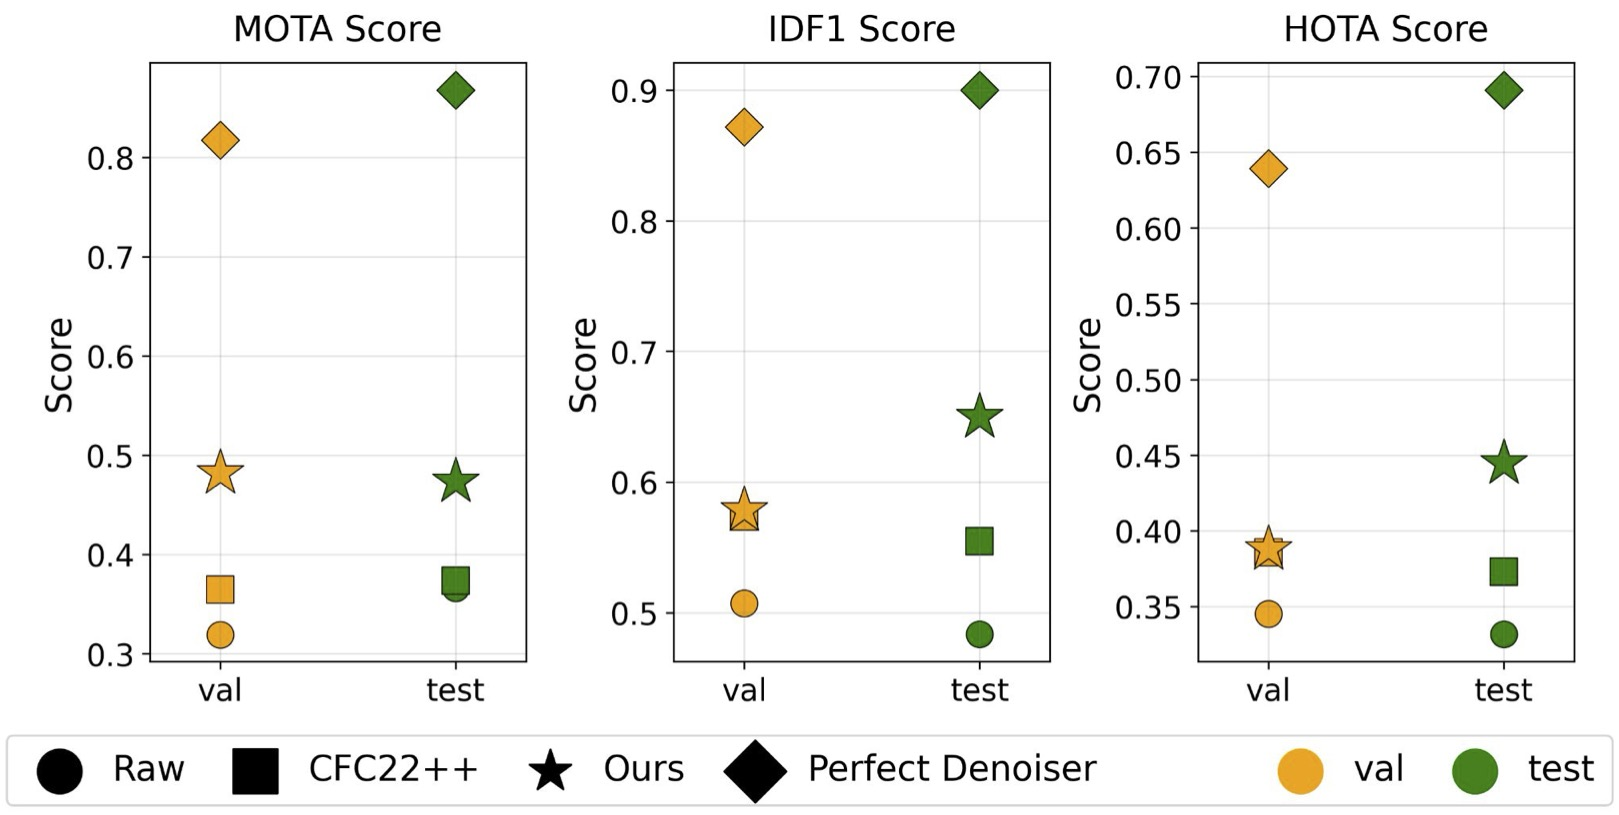
\includegraphics[width=\linewidth]{figs/tracking_scores.jpg}
    \caption{\textbf{Quantitative tracking improvements.} CFC22++ consists of the three-channel (background-subtracted, absolute-difference, raw) frames. The ``Perfect Denoiser'' refers to frames that have black backgrounds and white masks at the bounding box locations. Denoising results in higher MOTA scores for val and test; \NAME{} boosts IDF1 and HOTA scores in test moreso than in val.}
    \label{fig:track}
\end{figure}

% \vspace{-0.6in}

\subsection{Categorization Performance} 
\textbf{Lung Health Categorization: POCUS.}
Images processed through \NAME{} yield the best 5-fold cross-validation image classification score compared to classical and network-based denoising methods on lung categorization, shown in \cref{tab:big_table}. \cref{fig:covid} shows the precision-recall for the denoising methods on the Covid class -- \NAME{} has the highest accuracy for Covid classification. Additional per-class performance analysis is in Sec.\ \ref{sec:pocus_per_class_supp} of the Supp. mat.
\begin{figure}[tp]
    \centering
    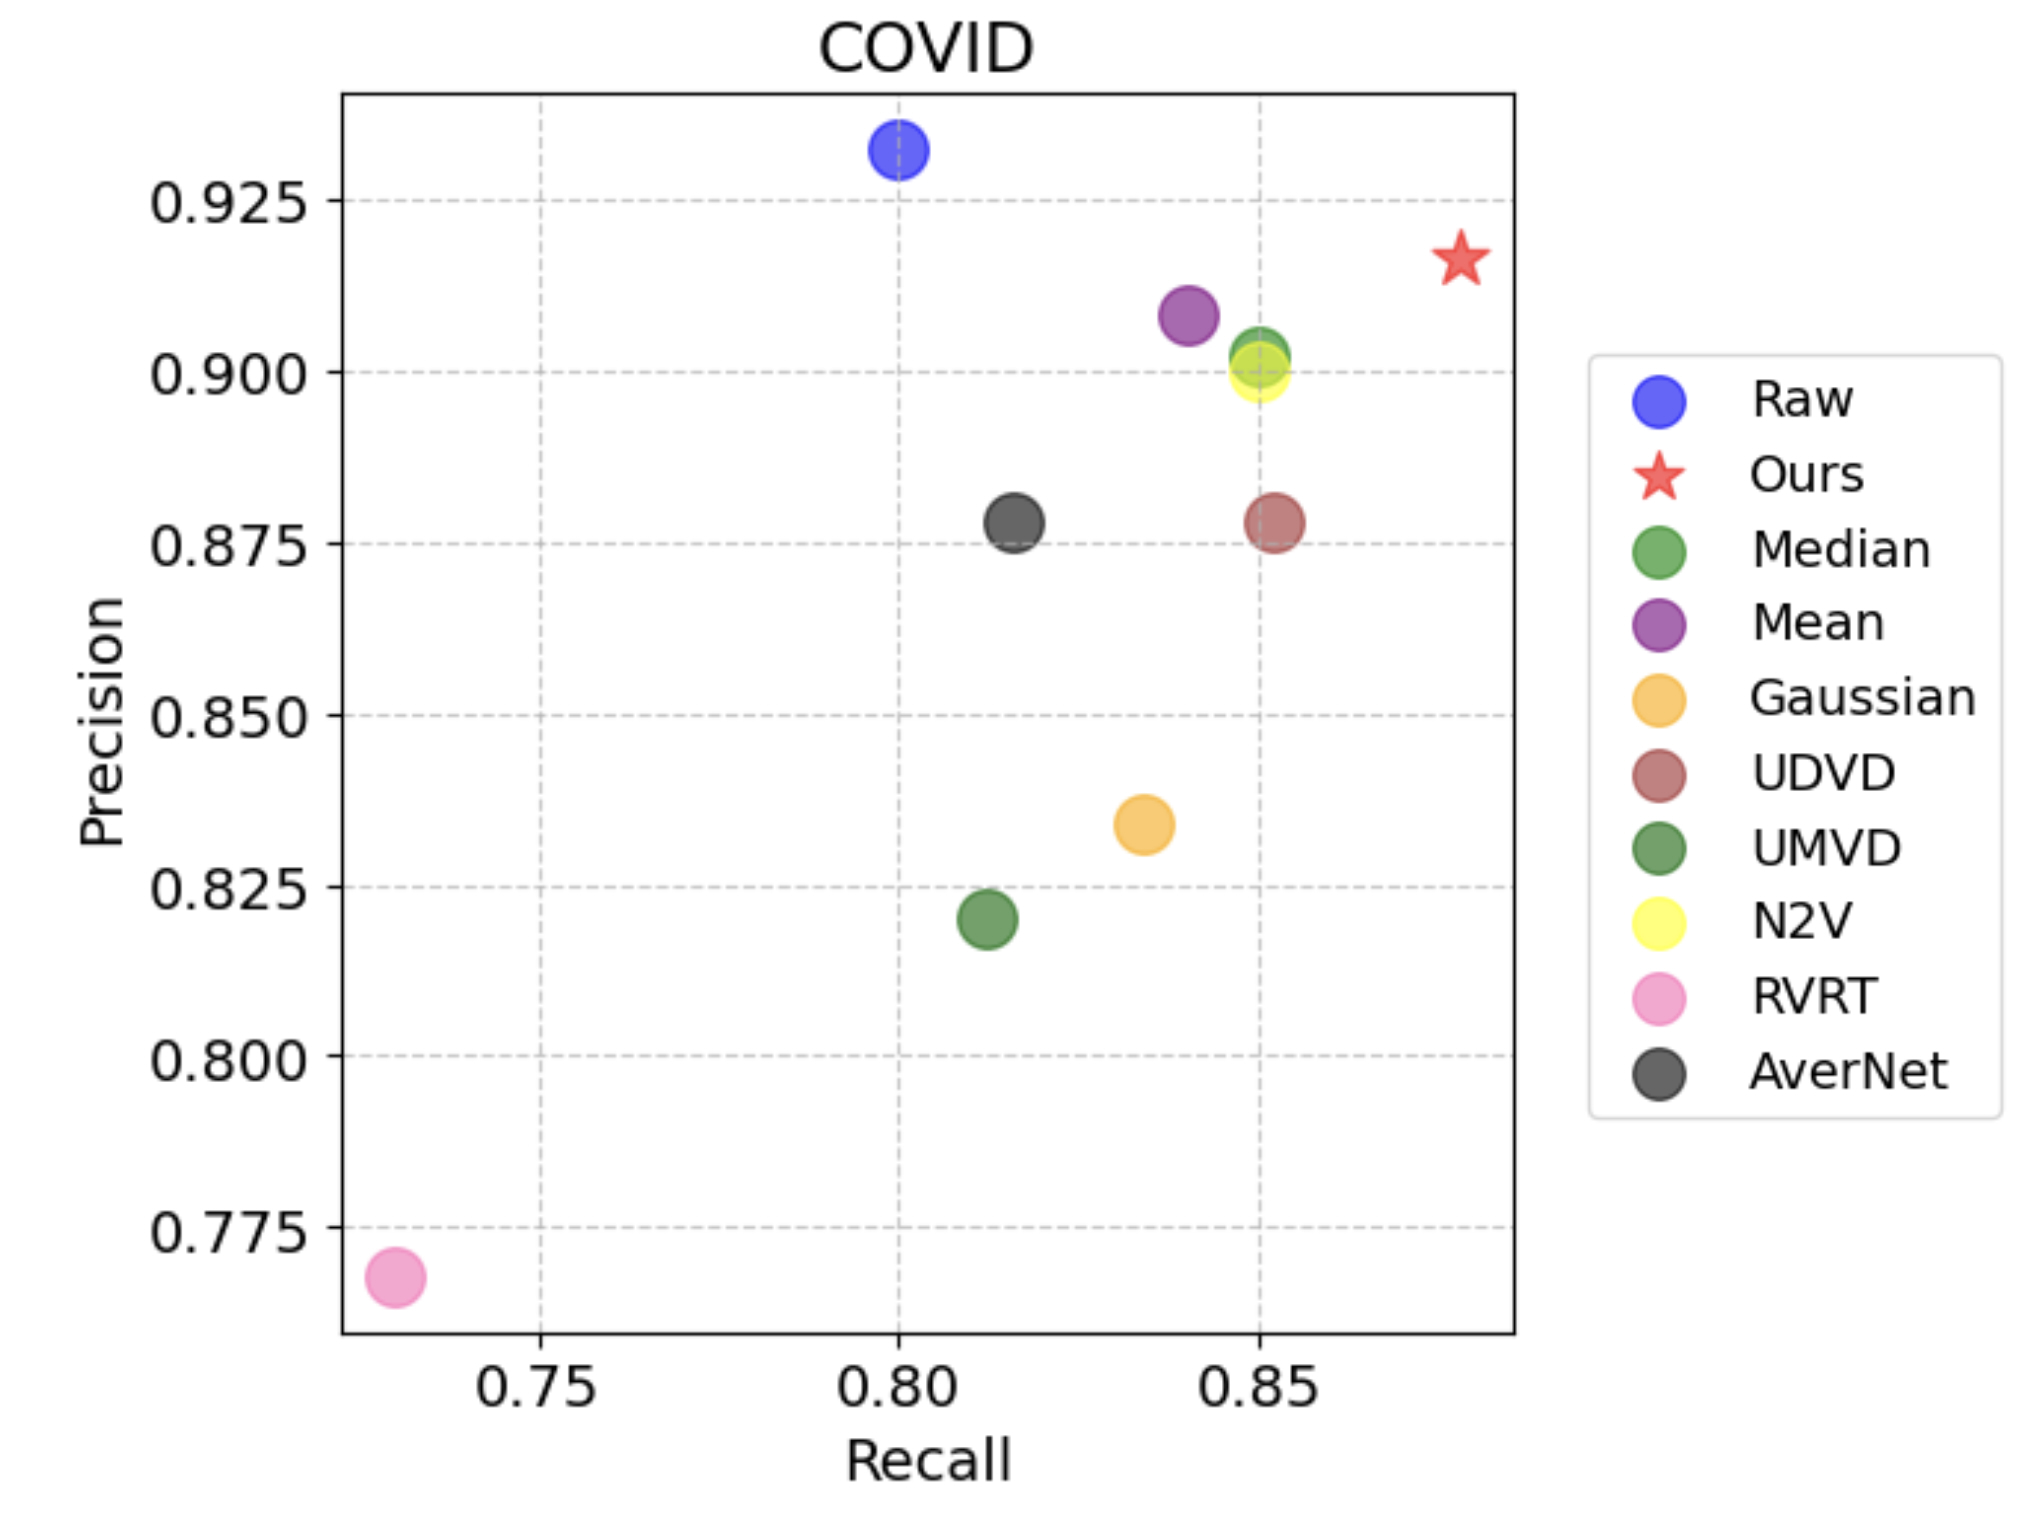
\includegraphics[width=0.75\linewidth]{figs/covid_pr_comparison_all_methods.jpg}
    \caption{\textbf{Covid Precision-Recall across denoising methods}. \NAME{} has the highest average precision and average recall across denoising methods. Additional class-wise performance comparisons are in \cref{fig:classwise_POCUS} in the Supplementary materials.}
    \label{fig:covid}
\end{figure}


\subsection{Ablations}
We ablate the reconstruction target and the denoising autoencoder to find their relative importance.

\noindent{}\textbf{Reconstruction Target}. PFDwT1 is the most effective reconstruction target for increasing the accuracy of downstream tasks. We compared PFDwT1 to PFDwT2, $\sigma$ (the standard deviation over input frames), $\Sigma-5\bar{I}$ (the sum of 5 consecutive frames - 5*mean frame), and $\Sigma-3\bar{I}$ (the sum of 3 consecutive frames - 3*mean frame). The results are shown in  \cref{tab:ablation_reconstruction_targets} and \cref{tab:targets} in the Supplementary material.

\noindent{}\textbf{Autoencoder vs. no Autoencoder}. Using a DAE improves downstream detection performance over using the reconstruction targets alone for all targets. More detail is in \cref{tab:ablation_reconstruction_targets} and \cref{tab:targets} in the Supplementary material.

% We conduct experiments on CFC22 (\cref{tab:ablations}) to understand the impact of the motion augmentation (reconstruction target, no denoising) vs. the impact of our method. We find the DAE improves performance for all train and test splits; for val splits, the DAE improves performance for all the $I_t$ reconstruction target. 

\noindent{}\textbf{Architectures} Our small architecture has better performance on downstream tasks compared to larger architectures. Comparisons of \NAME{} with a vanilla Autoencoder, a UNet\cite{unet}, and a UNet\cite{unet} with 3D convolutional kernels are shown in \cref{tab:big_table}. For additional details and architectures, see \cref{tab:additional_ablations} in the Supp. mat. The vanilla Autoencoder's architecture is also explicitly defined in \cref{tab:autoencoder_arch}.
% Autoencoder, the smallest architecture, outperforms UNet3D, the largest architecture on downstream CFC22 detection. Architectures based on resnet blocks and residual connections did not outperform our method architecture. Our DAE architecture yields the best performance, as shown in \cref{tab:big_table} and \cref{tab:architecture} in the Supplemental materials. Additional ablations are in \cref{tab:additional_ablations} in Supplemental materials.
% Additional ablations are in the Supplementary Materials.
% \subsection{Limitations}
